%%% LaTeX Template: Two column article
%%%
%%% Source: http://www.howtotex.com/
%%% Feel free to distribute this template, but please keep to referal to http://www.howtotex.com/ here.
%%% Date: February 2011

%%% Preamble
\documentclass[	DIV=calc,%
							paper=a4,%
							fontsize=11pt,%
							twocolumn]{scrartcl}	 					% KOMA-article class

\usepackage{lipsum}													% Package to create dummy text

\usepackage[english]{babel}										% English language/hyphenation
\usepackage[protrusion=true,expansion=true]{microtype}				% Better typography
\usepackage{amsmath,amsfonts,amsthm}					% Math packages
\usepackage[pdftex]{graphicx}									% Enable pdflatex
\usepackage[svgnames]{xcolor}									% Enabling colors by their 'svgnames'
\usepackage[hang, small,labelfont=bf,up,textfont=it,up]{caption}	% Custom captions under/above floats
\usepackage{epstopdf}												% Converts .eps to .pdf
\usepackage{subfig}													% Subfigures
\usepackage{booktabs}												% Nicer tables
\usepackage{fix-cm}													% Custom fontsizes
 \usepackage{amsmath}
 \usepackage{amssymb}
\usepackage{graphicx}

%%% Custom sectioning (sectsty package)
\usepackage{sectsty}			% Custom sectioning (see below)
\allsectionsfont{%			% Change font of al section commands
	\usefont{OT1}{phv}{b}{n}%	% bch-b-n: CharterBT-Bold font
	}

\sectionfont{%				% Change font of \section command
	\usefont{OT1}{phv}{b}{n}%	% bch-b-n: CharterBT-Bold font
	}



%%% Headers and footers
\usepackage{fancyhdr}			% Needed to define custom headers/footers
	\pagestyle{fancy}		% Enabling the custom headers/footers
\usepackage{lastpage}	

% Header (empty)
\lhead{}
\chead{}
\rhead{}
% Footer (you may change this to your own needs)
\lfoot{\footnotesize E: r.p.collins@sheffield.ac.uk}
\cfoot{}
\rfoot{\footnotesize page \thepage\ of \pageref{LastPage}}	% "Page 1 of 2"
\renewcommand{\headrulewidth}{0.0pt}
\renewcommand{\footrulewidth}{0.4pt}



%%% Creating an initial of the very first character of the content
\usepackage{lettrine}
\newcommand{\initial}[1]{%
     \lettrine[lines=3,lhang=0.3,nindent=0em]{
     				\color{Black}
     				{\textsf{#1}}}{}}



%%% Title, author and date metadata
\usepackage{titling}				% For custom titles

\newcommand{\HorRule}{\color{DarkBlue}%	% Creating a horizontal rule
				\rule{\linewidth}{2pt}%
		      }
%%begin novalidate
\pretitle{\vspace{-30pt} \begin{flushleft} \HorRule 
				\fontsize{25}{25} \usefont{OT1}{phv}{b}{n} 
\color{Blue} \selectfont 
				}
\title{In Pipe Repair of PE Pipe by Friction Stir Welding:\\
\huge{fixing without digging}}	

\posttitle{\par\end{flushleft}\vskip 0.5em}

\preauthor{\begin{flushleft}\large \lineskip 0.5em \usefont{OT1}{phv}{b}{sl} \color{DarkBlue}}
\author{Dr Richard Collins, }											% Author name goes here
\postauthor{\footnotesize \usefont{OT1}{phv}{m}{sl} \color{Black} 
					University of Sheffield, Sheffield Water Centre 								% Institution of author
					\par\end{flushleft}\HorRule}
%%end novalidate
\date{}																				% No date



%%% Begin document
\begin{document}
\maketitle
\thispagestyle{fancy} 			% Enabling the custom headers/footers for the first page 
% The first character should be within \initial{}

\initial{A} \textbf{significant cost of the repair of leaking pipes is in the locating and digging down to the level of the pipes.  
In addition there will be costs and reputation impacts due to the associated 
disruption, typically to road traffic.
A solution that allows the repair of pipes that doesn't require 
digging would, therefore, be a great advantage.  This proposal offers a design 
to allow the repair of PE pipes from inside the pipes, traversing from existing 
access points. By combining with existing sensing techniques it will allow the 
precise locating of leaks and assessment of the failure. In addition it will 
allow the post-installation verification and reassurance of joint viability, 
(both end joints and Top-Ts), a common cause of failure.}





\section*{Problem}
Polyethylene (PE) is the material of choice for the majority of pipe 
replacements due to its robustness and ability to be installed over long 
lengths. 
In general it suffers from a very low rate of failure compared to other materials. 
However, there exists clear evidence that there is significant leakage in MDPE 
mains laid by the UK water industry.
In 2010 UKWIR \cite{UKWIR2010} reported electro-fusion jointing as the predominant cause of joint failure on PE mains with a calculated failure rate of between 3 and 4 failures per 100 km per year. 
More recent data is hard to come by there is a widely held view within the industry that failure rates on PE mains have not reduced there is still a significant problem.



\section*{Proposed Solution}
The proposed solution technique involves developing a smart welding head that 
will be able to traverse along the inside of a pipe, detect and locate the leak 
or joint, and then weld the leak closed, or re-weld a joint using a Friction 
Stir Weld (FSW) process.

\subsection*{Leak / Joint Locating  and Assessment}
Accurately navigating in the pipe environment has been demonstrated at The 
University of Sheffield in the Assessing the Underworld Project 
\cite{ma2017pipeslam}. 
The project also demonstrated sensing of voids, leaks and other pipe 
defects using directed ultrasound.

\begin{figure}[htp]
 \centering
 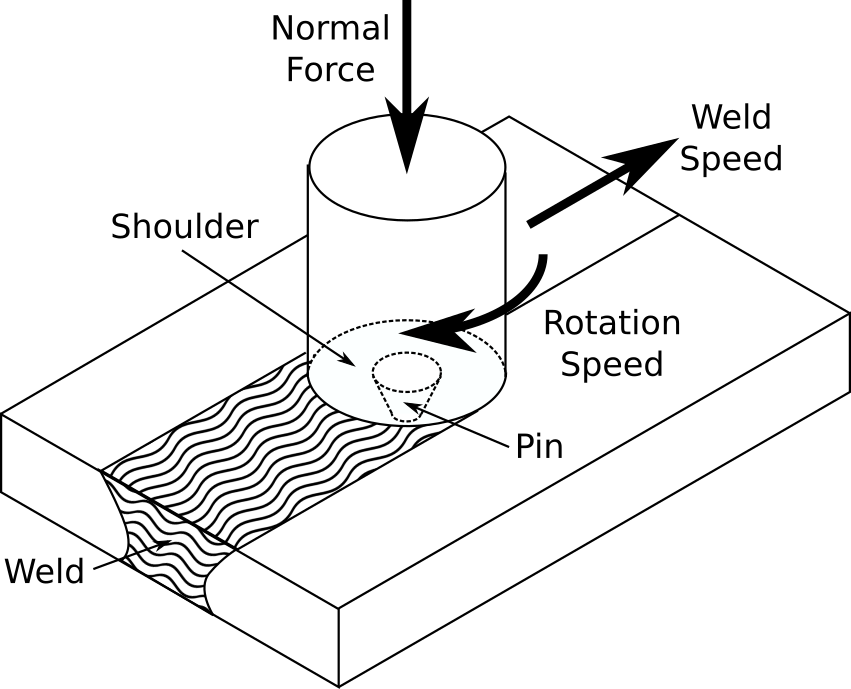
\includegraphics[width = 0.4\textwidth]{FrictionStirWeld}
 \caption{General friction stir welding process, the rotating tool (shoulder and 
pin) moves across the joint, mixing the material and forging with the frictional 
heat and pressure.}
 \label{FSWProcess}
\end{figure}

\subsection*{Friction Stir Welding}
Friction stir welding is a solid-state joining process that uses a 
non-consumable tool to join two workpieces \cite{mishra2005friction}. 
Heat is 
generated by friction between the rotating tool and the workpiece material, 
which leads to a softened region near the FSW tool. 
While the tool is traversed 
along the joint line, it mechanically intermixes the two pieces of material, and 
forges the hot and softened material by the mechanical pressure, which is 
applied by the tool, much like joining clay, or dough.




As can be seen in Figure \ref{FSWProcess} the working tool rotates and is passed 
across  weld line, the tool is comprised of two sections; the shoulder creates 
frictional heat, contains the softened material at the weld junction, and 
provides a suitable welding pressure,  the pin creates additional frictional 
head and directly stirs the materials together to form the weld.
Downward force is required to maintain the pressure on the joint and helps to create friction heat.


\subsubsection*{Friction Stir Welding of PE Pipes}
Whilst the majority of research into FSW has been undertaken on Aluminum and 
Steel, there have been a number of publications demonstrating its ability to 
join PE and other plastic sheets \cite{squeo2009friction,gao2014submerged}.  
In PE the FSW process directly mixes the chains of the polymers and has been 
demonstrated to produce a very strong joint \cite{zafar2017friction}.

\begin{figure}[htp]
 \centering
 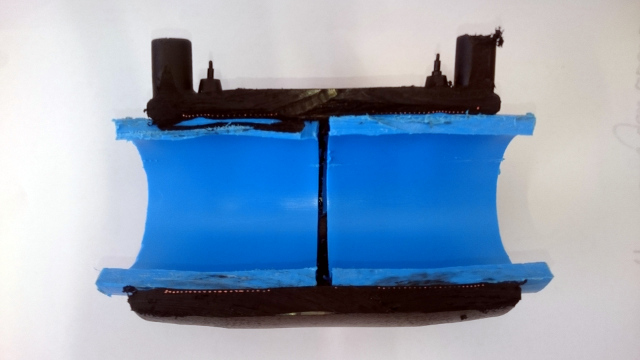
\includegraphics[width = 0.5\textwidth]{ElectroFusion}
 \caption{Section across an badly welded electro-fusion joint, the leak 
location can be seen on the top left where there is incomplete weld of the blue 
and black PE.}
\label{ElectroFusion}
\end{figure}

With FSW it is possible to weld both butted and lapped joints. As such it would 
be possible to fix leaks (butted joints), but also post installation re-weld an 
electro-fusion end joint (lapped and butted) or a Top-T (lapped). 
Figure \ref{ElectroFusion} shows a badly welded electrofusion joint, with the 
joint failure due to bad installation. The technique proposed here would allow 
for repair of sections such as this.

FSW is a particularly attractive solution as it should be possible to undertake 
a repair without de-watering the pipe \cite{gao2014submerged}.



\section*{Project Requirements}
The project is looking for an industrial partner to help support a funding 
proposal through Innovate UK\footnote{or direct industry funding} to 
demonstrate the viability of the FSW in pipe repairs.  FSW is a suitably mature 
technology that the research would not be in the fundamentals of the technique, 
rather in its co-option for in pipe repairs.


It is expected that the project would require to investigate:
\begin{itemize}
 \item optimal geometry of tool (shoulder and pin)
 \item optimal tool rotational speed, downward pressure to maximize the weld 
speed and strength
\item the strength and fatigue resistance of the resultant joints
\item the ability to miniaturize the weld head and provide suitable power and 
sensing capabilities
\end{itemize}

The successful demonstration of the technique would be achieved by the 
construction of a prototype smart welding head that was able to enter a pipe 
and traverse to a leaking section and undertake a repair weld.  This would be 
demonstrated using the new UKCRIC National Water Infrastructure
Facility: Distributed Water at the University of Sheffield.

The project is ideally suited to be undertaken at the University of Sheffield 
due to our extensive water laboratory facilities, background in water 
infrastructure assessment and history of projects exploring the fatigue effects 
on plastic joints.

\bibliographystyle{FG}
{\footnotesize
\bibliography{FSW}}



\end{document}